\subsection{Distributed Denial of Service (DDoS)}
\label{subsec:03_ddos}

% TODO add an army of zombies

% Introduction describing the base of such attacks
A DDoS (Distributed Denial of Service) attack has become a popular way to cripple a server of an institution or a private person and has shown to be an immense threat to the Internet. However, how is it possible for attackers to execute such attacks? The current internet design has its purpose of moving packets from a source to a known destination. The network itself minimally forwards all packages at minimal cost and generally outsources the complexity, including security, transport reliability and quality of service to the sender and receiver of the transported packages. This concept has been called the \textbf{end-to-end paradigm}. As no intermediary entity will step in, a party (either sender or receiver) can damage its opposition by using different attack possibilities such as IP Spoofing or the aforementioned DDoS attacks \cite{Mirkovic2004}. By faking the source address in the header of a packet, the sender can hide its identity. This security issue is called IP Spoofing \cite{Cloudflare2019}. As described in \citet{Mirkovic2004} following security issues raise opportunities of attacks:
\begin{itemize}
    \item Limited internet resources: Every host or service has hardware limitations that users may consume.
    \item Highly interdependent internet security: No matter how secure a host may be configured, DDoS attacks always depend on the security of others within the Internet.
    \item No collocation of intelligence and resources: The intermediate network has plentiful resources, as they forward package at minimal costs.  In contrast, the end networks only invest in as much bandwidth as they planned to use for their services.
    \item No enforcement of accountability: As described above, attackers can escape from accountability by using IP Spoofing mechanisms.
    \item Distribution of control: In a world of a distributed network, such as the Internet, multiple clients participate in that network. Each one of them has different security mechanisms. No global control entity can define a security policy or standard.
\end{itemize}
% Additional reasons/base of attacks
Since the number of connected devices has increased due to IoT devices such as connected cameras, or smart fridges, attackers have a growing capacity to take control of unsecured devices \cite{Rodrigues2017a}.

% Explaining DDoS
By deploying multiple attacking entities, attackers using DDoS try to overflood a service provisioning or other published web applications and prevent rightful users from accessing the application. More precisely, attackers send a stream of packets to the victims, which consume all capacity of hardware resources and therefore make it unavailable for legitimate clients to access the service provider. Another popular way for an attacker is to send malformed packets to shut down the availability of the application service. Those packets confuse the web application or some protocols on the victims' hardware and force the server to reboot. There are probably some additional possibilities to shut down services on the internet. Such attack possibilities will be discovered first when they have been exploited in a significant attack and servers have been down for a particular time \cite{Mirkovic2004}.

% DDoS procedure
The procedure of a DDoS attack is split into the following phases: An attacker recruits multiple agents (clients) into which the attacker injects malicious code. Attackers often hide the identity of infected clients by using IP Spoofing mechanisms \cite{Mirkovic2004}.

% TODO Difference DoS and DDoS?

% TODO Motivation behind DDoS
Multiple incentives exist to attack clients using DDoS attacks. Unfortunately, the primary goal of such an attack is to damage the selected victim. The motives may be found in prestige (gaining respect within the hacker community when attacking popular websites or services), personal hatreds, material gain (damaging competitors by attacking them), any political reasons or merely blackmailing others \cite{Mansfield-Devine2015, Mirkovic2004}.

% TODO generalize possibilities of mitigation strategies

Various companies (known from other services) currently offer DDoS protection services, such as Cloudflare or Akami, and its number is increasing \cite{Pras2016}. For all solutions, a third party DDoS Protection Service (DPS) provider is required, resulting in extra costs, as the analysis performs in the cloud \cite{Rodrigues2017}. By utilizing resources from other companies, any difficulty of mitigating DDoS attacks can be shared \cite{Rodrigues2017}.

% TODO More about DOTS (DDoS Open Threat Signaling) an IETF proposal
% TODO probably explain Gladius?
The Internet Engineering Task Force (IETF) additionally is proposing a protocol called DOTS (DDos Open Threat Signaling) that requires both client and server. A new protocol is required which has to be maintained. DOTS clients have to register to a DOTS server and use this protocol among the agents to organize the DDoS protection \cite{Rodrigues2017a}. In the following sections, various approaches to mitigating DDoS attacks are illustrated as seen in popular papers without the need to deploy a new protocol.

\subsubsection{DDos Mitigation with Smart Contracts}
% \cite{Rodrigues2017}
This concept investigates a possibility to mitigate a DDoS attack in a fully decentralized manner using smart contracts and their underlying technology Blockchain. Those technologies allow sharing information (detection and mitigation mechanisms as well as IP addresses) about attacks in an automated and decentralized system \cite{Rodrigues2017}.

As described in \ref{subsec:02_smart_contracts} a smart contract is a software that is made to help contracts being able to execute and verify on its own. To do so, there has to be an infrastructure that implements, verifies and enforces the negotiation of those smart contracts by using particular computer protocols and that runs fully decentralized. As known from \ref{subsec:02_blockchain}, a blockchain ensures permanent storage and provides obstacles to manipulate content and is thus an ideal infrastructure for smart contracts. Nodes participating in the blockchain run a smart contract by executing and validating a script and thereafter storing the contract and the results in a new block \cite{Rodrigues2017}.

% Proposed System Architecture
As presented in \ref{system_architecture} the architecture is composed of three components. The customers report IP addresses to the blockchain via smart contracts. The autonomous systems (AS) retrieve lists containing these addresses and implement DDoS mitigation techniques. All participants interact with the underlying technology of blockchain \cite{Rodrigues2017}.

The web server of one autonomous system (AS) is a victim of a DDoS attack. Participants, that have proven ownership of their IP,  then create a smart contract that stores all IP addresses of attackers. Subscribed systems receive updated lists of IP addresses every 14 seconds, as this approaches underlying blockchain technology, Ethereum, creates new blocks within that timeframe. As soon as all other autonomous systems receive the attackers' list, various mitigation strategies may be triggered individualized to the specific domain \cite{Rodrigues2017}.
\begin{figure}[ht]
  \begin{center}
  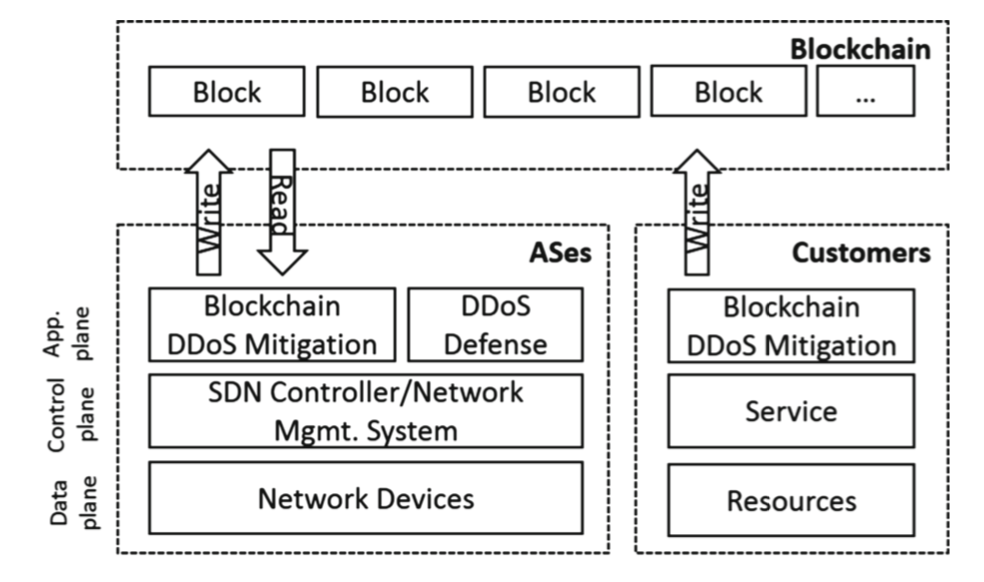
\includegraphics[scale=0.6]{Talk7/img/ddos/collaborative_ddos_mitigation_system_architecture}
  \end{center}
  \caption{System Architecture}
  \label{system_architecture}
\end{figure}

% Conclusion
To summarize, this approach uses an already existing and publicly available distributed infrastructure to adumbrate IP addresses that are either white- or blacklisted. This approach serves well as an additional security mechanism to existing DDoS defense systems across multiple domains by using an Ethereum blockchain without transferring the control of their internal network to a third party. For large-scale attacks, this approach currently is not supported well, but this issue will be addressed in the future work of this approach \cite{Rodrigues2017}.


\subsubsection{Mitigation-as-a-service in cooperative network defenses}
% \cite{Mannhart2018}
% Short introduction
With cooperation between multiple domains, various collaborating Autonomous Systems (AS) can alleviate DDoS attacks by redirecting excessive traffic to other domains for filtering the traffic.

As soon as a target AS detects an attack, the target sends a request to all participating AS's to mitigate the current attack. Subsequent, a mitigator AS, which is responsible for the range being attacked then either accepts or declines the mitigation request. By using a proof-of-mitigation, the completion of the mitigation has to be confirmed, and the target can pay the mitigator. As this proof-of-mitigation has to satisfy constraints of time, tamper-evidence, and reproducibility this proof has to be executed automatically during the current time window. Additionally, any user interaction has to be excluded to ensure efficiency \cite{Mannhart2018}. Various approaches creating such proof will be described and discussed in this section. It will be shown that no individual approach could be used to address a trade-off between practicability and security.

\paragraph{Marketplace of Mitigation VNFs}
Virtualized  Network Functions (VNF) can be deployed on any hardware. The concept of Network Function Virtualization (NFV) can, therefore, provide an efficient solution for deploying these VNFs by virtualizing a single function in the network. All ASes involved in the cooperative network could load the VNF image directly from the marketplace, which then provides the mitigation service. By comparing the hashed checksum of the VNF image to a known value from the marketplace, the integrity of the VNF image will be checked. Local caching of all VNFs avoids large load on the marketplace. A big advantage of this approach is the high degree of isolation, as the VNFs consists of the minimal code which is necessary to handle the mitigation. Additionally, the VNFs can be set up on any hardware without any additional configurations. Unfortunately, the target still needs to trust that the mitigator only runs untampered VNFs directly from the marketplace \cite{Mannhart2018}.
% TODO overwork
\begin{figure}[ht]
  \begin{center}
  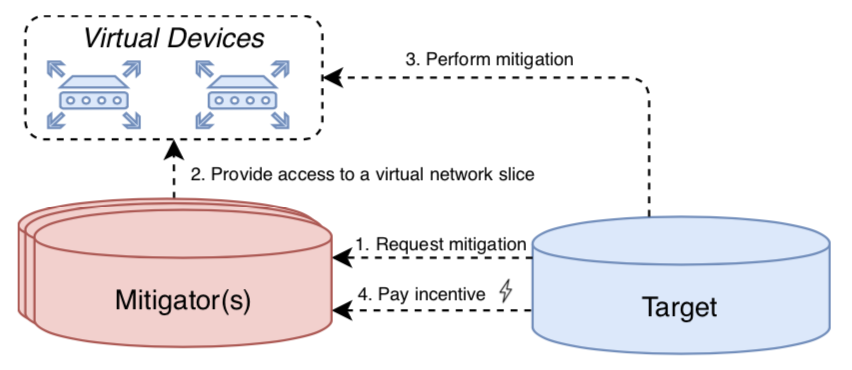
\includegraphics[scale=0.5]{Talk7/img/ddos/cooperative_network_marketplace_vnfs}
  \end{center}
  \caption{Marketplace of Mitigation VNFs}
  \label{ddos_marketplace_vnf}
\end{figure}

\paragraph{Trusted Computing}
So-called Trusted Platform Modules (TPM) allow secure storage of hashes that verify in the on-chip Platform Configuration Registers (PCR) that attest secure boot chain from BIOS over Bootloader. By using this approach, only the code that is approved by the cooperative defense will be run on the system. VNFs create a defense network where trusted and known VNFs always handle requests for mitigation without trusting the responsible operator that provides the mitigation service to the AS.  A big disadvantage of trusted computing is the strict hardware requirement, as the TPM is only available as a standalone chip or integrated into the motherboard.
\begin{figure}[ht]
  \begin{center}
  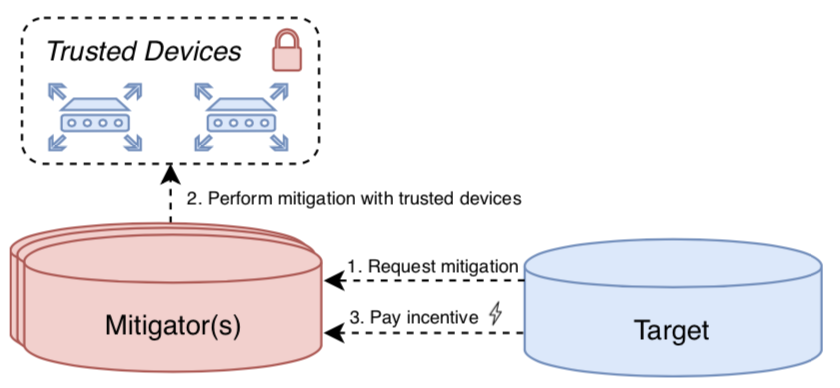
\includegraphics[scale=0.5]{Talk7/img/ddos/cooperative_network_trusted_computing}
  \end{center}
  \caption{Trusted computing}
  \label{ddos_trusted_computing}
\end{figure}

\paragraph{Secure logging}
As the mitigators can use full network infrastructure, they are allowed to create a proof of mitigation using the available traffic data. By having a detailed log of network activities, they could prove the successful mitigation by identifying a reduction in the traffic from the attack source to the DDoS target. A mitigation-proof based on the log files decreases the complexity of the proof. The aforementioned log file has been created on an isolated system and therefore has to be checked about its integrity by a third party. A disadvantage comes with high-volume attacks which create large log files. These large files introduce additional delays as the log files have to be transferred for remote auditing.
\begin{figure}[ht]
  \begin{center}
  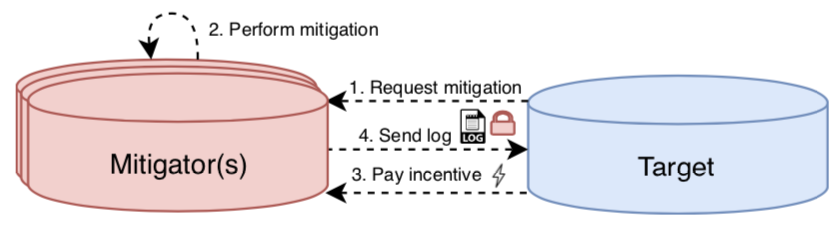
\includegraphics[scale=0.5]{Talk7/img/ddos/cooperative_network_secure_logging}
  \end{center}
  \caption{Secure logging}
  \label{ddos_secure_logging}
\end{figure}
% TODO

\paragraph{Network Slicing}
Since network virtualization technologies and Software-Defined Networks (SDN) have advanced in recent times, they both serve as a basis for network slicing as a service. When the attack target AS requests mitigation services, it gains access to the virtualized network slice of the mitigator AS. The slice is then configured to provide access for all attacking IP addresses that have been requested within the mitigation request.
\begin{figure}[ht]
  \begin{center}
  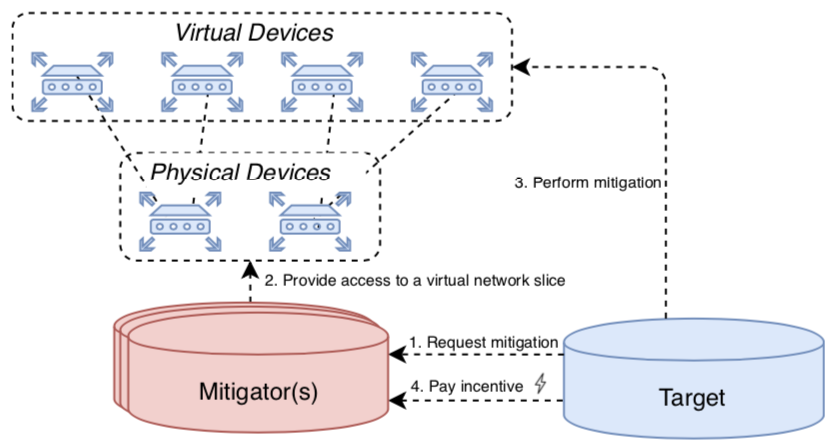
\includegraphics[scale=0.5]{Talk7/img/ddos/cooperative_network_network_slicing}
  \end{center}
  \caption{Network Slicing}
  \label{ddos_network_slicing}
\end{figure}

% Final considerations of this paper?

\subsubsection{Multi domain DDoS Mitigation based on blockchains}
% \cite{Rodrigues2017a}
Another approach again uses smart contracts and therefore blockchain as a mean to advertise information across multiple domains. The architecture as seen in figure \ref{ddos_multi_domain_architecture} involves the following entities: \textbf{Software-Defined Networks (SDN)} enable the development of customizable security management. A \textbf{Network Function Virtualization (NFV)} enforces the security policies through virtualized functions. An Ethereum-based \textbf{blockchain} is a base for all participants of the cooperative network to advertise DDoS attacks within a timeframe of 14s, as a new block is mined within that time. At last a \textbf{smart Contracts} which is storing black or whitelisted IP addresses of customers.

\begin{figure}[ht]
  \begin{center}
  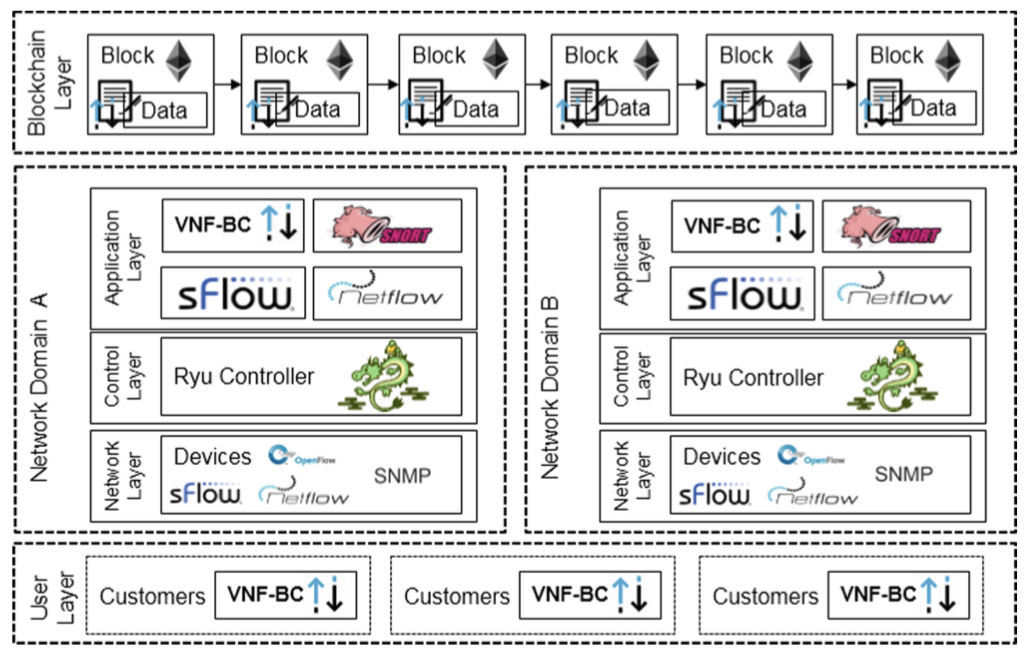
\includegraphics[scale=0.5]{Talk7/img/ddos/multi_domain}
  \end{center}
  \caption{Multi-domain architecture}
  \label{ddos_multi_domain_architecture}
\end{figure}

% TODO conclusion of paper?

\subsubsection{Blockchain Signaling System (BloSS)}
% https://github.com/blockchain-signaling-system/bloss-core
% https://github.com/savf/BloSS
% \cite{Rodrigues2019}

Similarly to \cite{Rodrigues2017a}, this paper deals with cooperative, multi-domain DDoS defense systems, but it presents a Blockchain Signaling System (BloSS) which is a somewhat technical approach of deploying hardware simplifying signals of DDoS attacks. Principal components for a BloSS are smart contracts that describe how information has to be transferred between Autonomous Systems (AS) and decentralized applications that include parameters defining the interaction of AS. Additionally, a consortium based blockchain, differentiating from the public and private blockchains, serves as an intermediary level of confidence. An Autonomous System (AS) thereby creates a wallet and notifies a smart contract that stores some information. The smart contract then implements a method to reclaim addresses published by other systems by querying a central smart contract. This central SC is used to configure all involved smart contracts with updated information on their managed IP networks, as the addresses of the involved wallets are immutable. In order to prevent free-riding peers (parties that only consume without any contribution), an incentive mechanism need to be set by defining tokens.  % TODO what do they do?
%  TODO more about Architecture and Hardware?
